\documentclass[a4paper,11pt]{article}
\usepackage{pagecolor,lipsum}
\usepackage{hyperref}
\definecolor{LinkColor}{HTML}{FBF1C7}
\usepackage[francais]{babel}
\usepackage{xpatch}
\usepackage{fdsymbol}
\usepackage{graphicx}
\hypersetup{
    colorlinks,
    linkcolor={LinkColor},
    citecolor={LinkColor},
    urlcolor={LinkColor}
}
\definecolor{BlackHaf}{HTML}{101213}
\definecolor{WhiteHaf}{HTML}{EEEEEE}
\definecolor{LightOrangeHaf}{HTML}{C5A782}
\definecolor{OrangeHaf}{HTML}{DA8548}
\newcommand{\e}{\'{e}}
\makeatletter
\newcommand{\globalcolor}[1]{%
  \color{#1}\global\let\default@color\current@color
}
\makeatother
\AtBeginDocument{\globalcolor{WhiteHaf}}
\title{\color{OrangeHaf} Par Philipe langevin}
\date{}
\begin{document}
\pagecolor{BlackHaf}
     \begin{center}
     \hfill
\includegraphics[width=9cm]{dragon.png}\hspace*{\fill}
     \\
     \textbf{\color{OrangeHaf}\huge Theorie des langages}\\
     \text{Note de T.Hafsaoui}
     \\
     \text{rours de Nicolas Meloni 2021}
     \end{center}
     \tableofcontents
    \section{\color{OrangeHaf} Chapitre 0: Une premiere approche du compilateur}
     \subsection{Introduction}
        En informatique en generale, et tout particulierement dans la sciences de l'informatique
        on suit une logique similaire celle ci ce decompose de cette maniere pour notre tres chere compilateur.
        \begin{enumerate}
            \item Theorie mathématiques: theorie des langage
            \item Modelisation ou traduction du probleme en struture de donnees informatique: arbre,graphe
            \item Toruver un algorithme efficace afin de resoudre nos probleme
            \item Programmation
        \end{enumerate}
        Le cours est baser sur la bible de la compilation "$Le\ Dragon$"(Compilation :Principes, technique et outils).
     \subsection{Historique}
        L'Histoire des compilateur commence en 1950 precedament les programmes etait ecrit en langage machine avec les inconenients que cela accompagne.\\
        Le premier compilateur est ecrit par Grace Hopper pour le langage A, divers linguiste et Knuth aurons aussi un role important dans nos compilateur moderne avec par exemple $GCC$(GNU compiler collection) comme aboutisment, qui aujaud'hui compile pas moins de 7 langage dont le C et fait meme le cafe.
        \\
      \subsection{Une rapide presentation}
\begin{center}
      \textbf{\color{LightOrangeHaf}Compilateur:}
          Un compilateur est esentiellement un traducteur, il prend en entree un programme ecrit dans un langage $L1$ et produit un programme \underline{equivalent} dans un langage $L2$.\\
          L'usage veut que le programme en sortie soit en langage machine, c'est a dire executable par la machine.
    \end{center}
    On peut distinguer deux familles de compilateur:
    \begin{enumerate}
      \item Compilateur(les \textbf{vrai})\\ Produit du code machine dont l'execution se fait ulterieurement avec des donnees
      \item Interpreteur\\ Lit le programme et effectue lui meme les opration sur les donnees.
    \begin{center}
     \hfill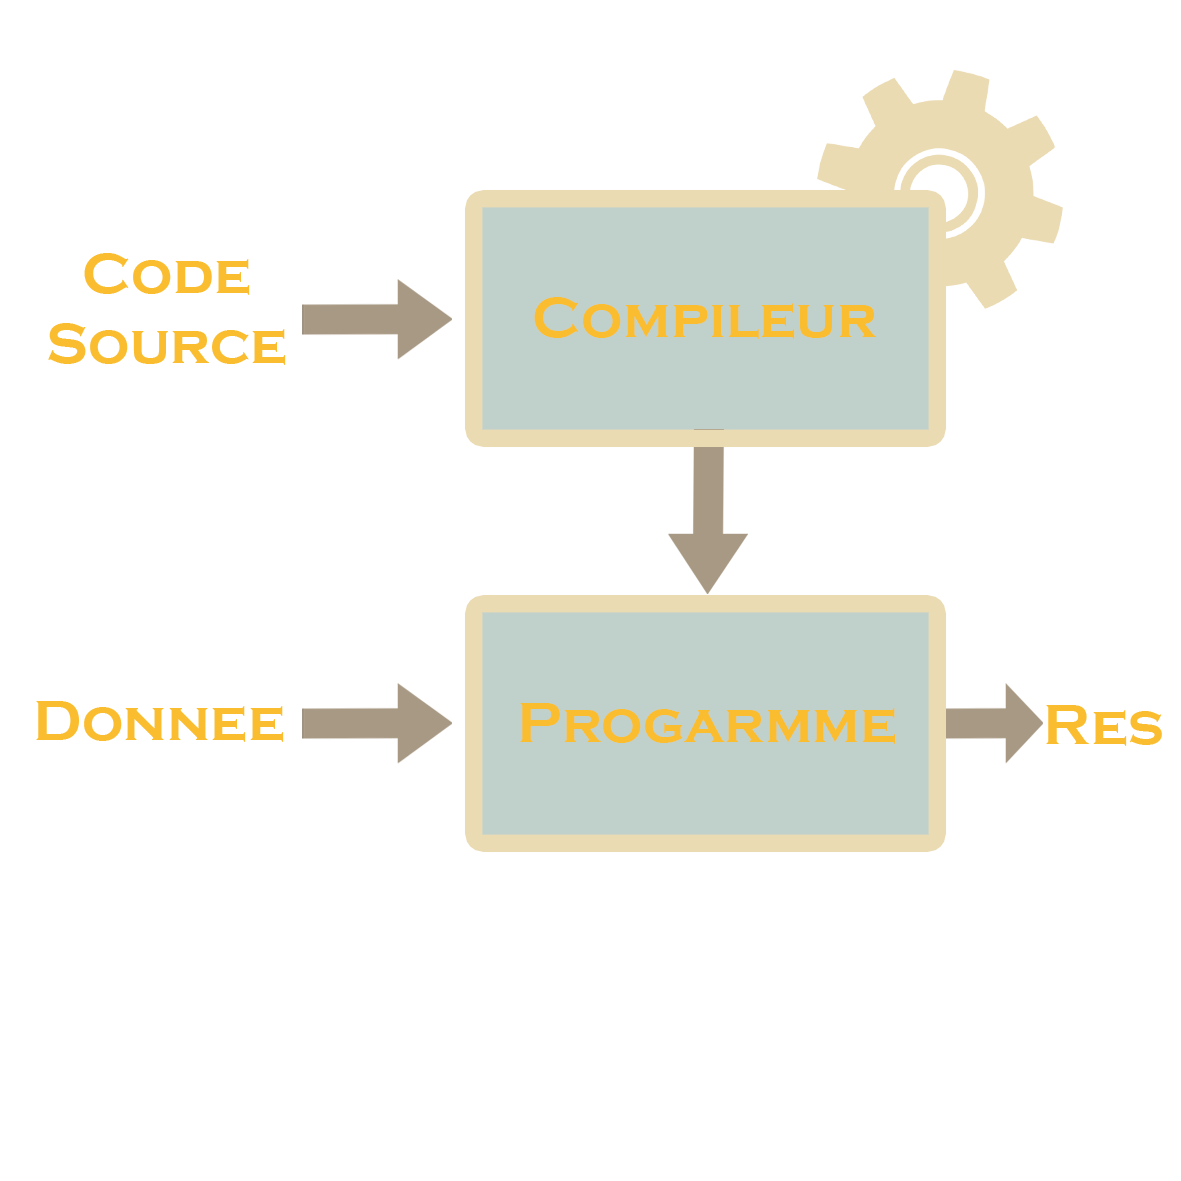
\includegraphics[width=7cm]{fig1.png}\hspace*{\fill}
    \end{center}
    \end{enumerate}
    En generale le compilateur produit du code de maniere plus efficace(vitesse,taille,consomation memoire/electrique).
    En effet au contraire du compilateur il peut prendre la totalite du code source comme base de travaille et faire des optimisation de maniere globale, ce qu'evidament un interpreteur ne peut faire.\\
    remarque: Un programme C est, en generale, 10x plus rapide que sont equivalent en python.\\

    On parle souvent de langage compiler ou interpreter mais il s'agit d'un abus de langage. Un langage de programmation est avant tout une norme tout language peut donc etre compiler ou interpreter.
    \subsubsection{Bootstrapping}
    Le compilateur C $gcc$ est ecrit de maniere asser peut intuitive en\dots C.
    On se retouve donc fasse a un probleme d'oeuf et de poul, on parle dans ce cas la de probleme de $Bootstrapping$ ou amorcage dans la langue de Moliere.
    Pour resoudre ce probleme on ecrit un premier compilateur en langage machine pour un sous-ensemble du C, puis on etend succesivment le compilateur a tout le language a l'aide des compilateur intermediaire.
    \begin{center}
      Appelons $C_1$ $C_2$\ldots $C_n$ les sous ensemble de C:\\
     \hfill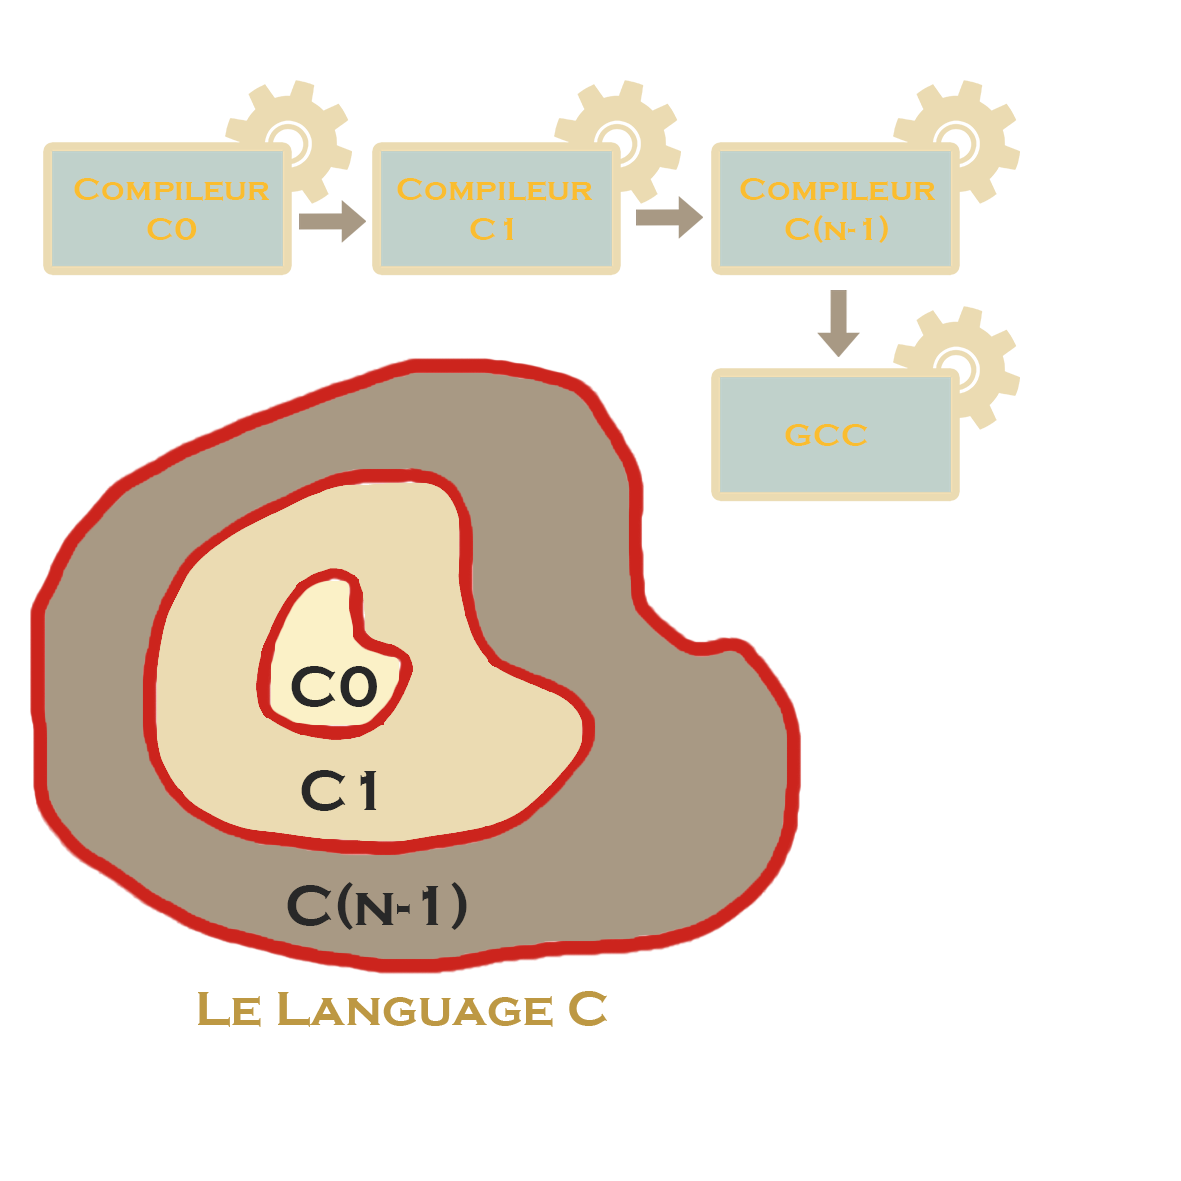
\includegraphics[width=8cm]{fig2.png}\hspace*{\fill}
    \end{center}
    A la fin lorsque l'ont se retouve avec un compilateur C ecrit en langage $C_{n-1}$ on peut enfin ecrire un compilateur C.
    \subsection{Exemple de compilation}
      \subsubsection{Python}
      \noindent\begin{minipage}{0.4\textwidth}% adapt widths of minipages to your needs
    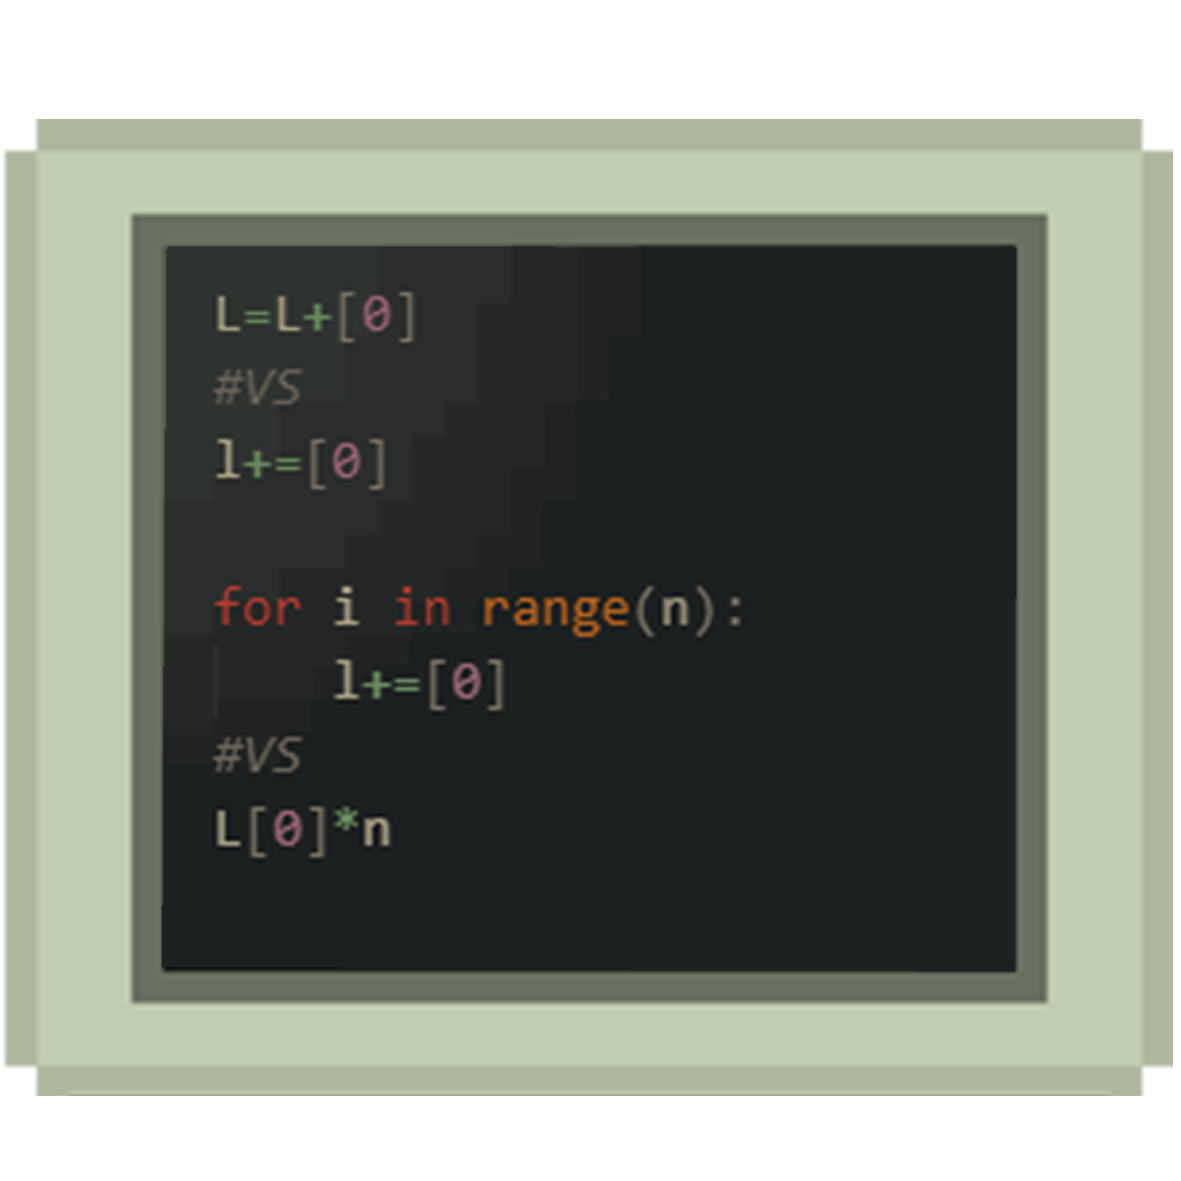
\includegraphics[width=\linewidth]{fig3.png}
    \end{minipage}%
  \hfill%
  \begin{minipage}{0.5\textwidth}\raggedleft
    Lors de l'execution d'un scripte, l'interprete compile les instruction en $Bytecode$(langage de la machine virtuelle de python), la machine virtuelle execute ensuite le bytecode.\\
        En generale le processus produit un fichier en .Pyc(python compiler), ce fichier permettra une execution plus rapide en cas de $2^{nd}$ utulisation.
        Le module $dis$(pour disambleur) peremet d'obtenire le $Bytecode$ d'un scripte. On peut ainssi de cette maniere etudier la difference d'efficacite entre deux methode.
  \end{minipage}
  \subsubsection{C}
    La compilation avec $GCC$ se fait en 4 phase:\\
    \begin{itemize}
      \item \underline{Prepoceseur:}Le fichier source est analyse et des transformation textuelle sont effectue (\# define, \# include, \# ifdef).
      \item \underline{Compilation:}Traduction en assembleur (verification de la norme du langages).
      \item \underline{Assemblage}traduction en langages machine(fichier en .O)
      \item \underline{Edition de lien}Les fichier sont lier entre eux pour produire l'executable.
    \end{itemize}
    Les option -E, -S, -c permete l'arret de la compilation a chacune de ces phases.
  \subsection{L'outils Make}
  C'est un outils de generation de fichier, en generale l'outils se presente sous forme de regle dans un fichier nommer $Makefile$ ou $makefile$. C'est regle sont constitueer d'une serie d'instruction sous la forme:\\
  \begin{center}
    \color{OrangeHaf}Cible : \color{LightOrangeHaf} dependance 1\ldots dependance n\\
            Commande
  \end{center}
  Lors de l'execution de la commande $make$ l'outils analyse les commande succesive, les regle et surtout les date de derniere modification des dependance.
  Si l'une de ces date est plus recente que celle de ca cible $make$ execute les differente instruction afin de mettre a jour la cible.\\
  Petite exemple:
  \begin{center}
    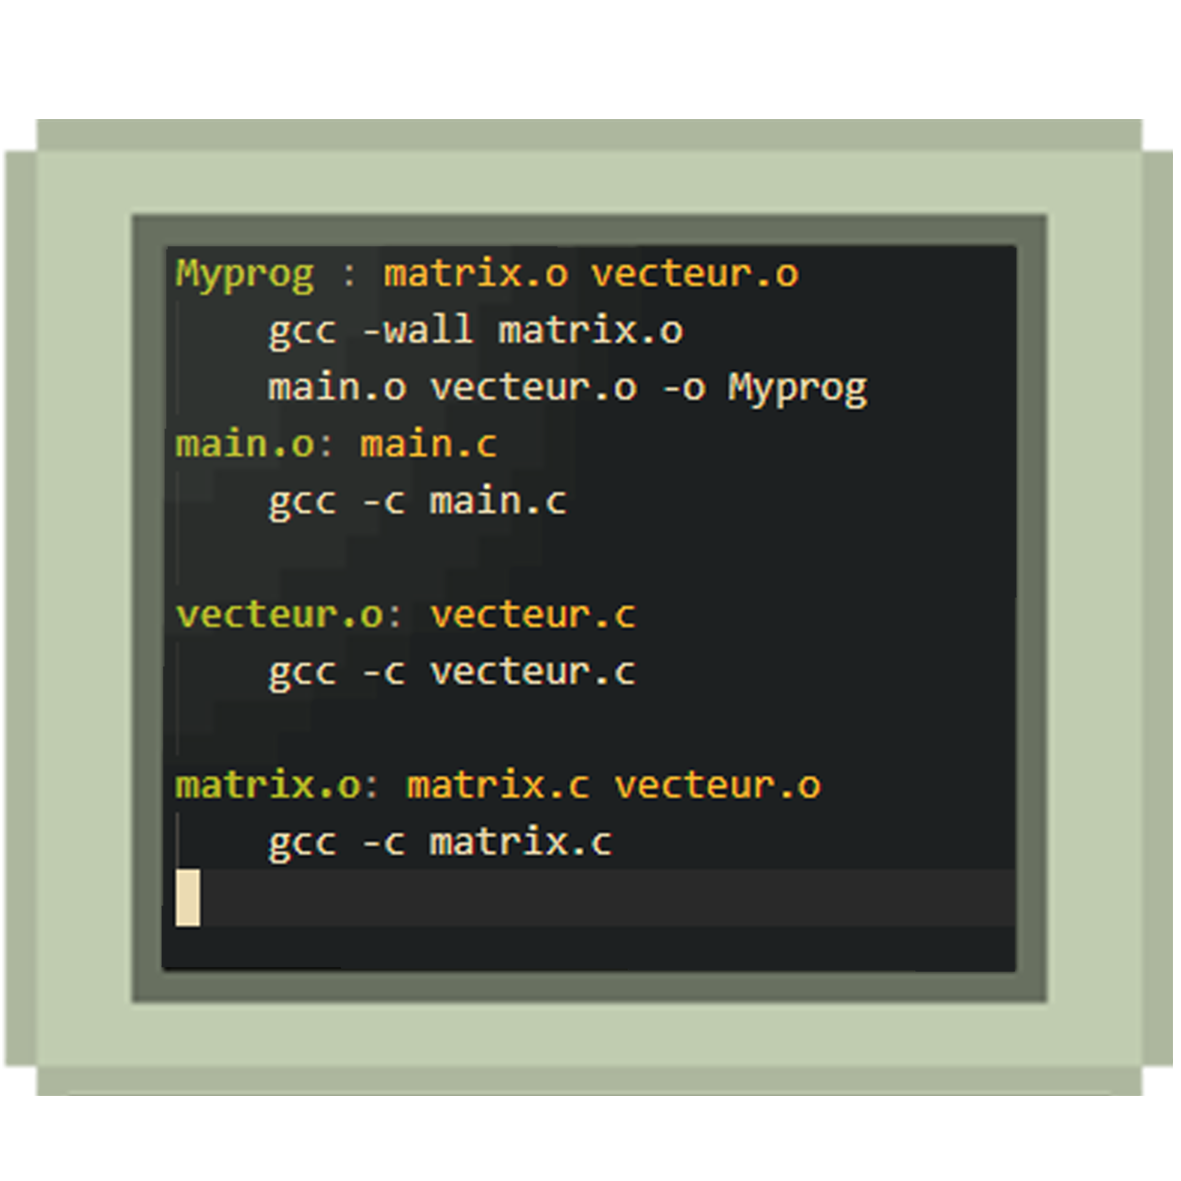
\includegraphics[width=7cm]{fig4.png}
  \end{center}
  \begin{itemize}
    \item Cas 1: Lors du premier appel a $make$ l'outils cree tous les fichier .o puis le programme Myprog.
    \item Cas 2: Tout est compiler mais main.c, et modifier seule la commande qui concerne la cible $main.o$ et $Myprog$ seront de nouveaux executer.
    \item Cas 3:On modifie vecteur.c avec tout deja compiler. De maniere logique vecteur.o matrix. et $Myprog$ seront recompiler.
  \end{itemize}
  \textbf{Tips:} Il est possible de simplifier l'ecriture des makefile on autorise l'utulisation de variable et de racourcis. Ici une variable permet simplement de donner un nom a une chaine de chractere:
  \begin{center}
  \color{OrangeHaf}Non\_de\_chaine=\color{LightOrangeHaf} \$(chaine de char)\\
  \end{center}
  Il existe aussi des variable predefinie:
  \begin{itemize}
    \item \$@: le nom de la cible
    \item \$\^: ensemble de dependance
    \item \$$<$: premiere dependance
  \end{itemize}
  \textbf{Cible Phony:} Il est possible de simplifier l'ecriture des makefile on autorise l'utulisation de variable et de racourcis. Ici une variable permet simplement de donner un nom a une chaine de chractere:
  \begin{center}
    \color{OrangeHaf}Clean:\\
      \hspace{\parindent} \hspace{\parindent} \hspace{\parindent} \hspace{\parindent} \hspace{\parindent} \hspace{\parindent} \hspace{\parindent} \hspace{\parindent} \hspace{\parindent} \hspace{\parindent} \hspace{\parindent} \hspace{\parindent} \color{LightOrangeHaf} rm -f *.o *~
  \end{center}
  \subsection{Structure d'un compilateur}
  On peut decompose le processus de de compilaction en 2 grande phase:
  \begin{enumerate}
    \item \textbf{L'analyse}(Partie frontal):\\
          qui consiste a construire une representation abstraite du programme afin d'en degager la structure gramatical. Il s'agit d'extraire du flot de donnees en entre les different composant et de les relier entre eux en fonction de la grammaire.
    \item \textbf{La synthese}(Partie final):\\
          se serre des donnees de l'analyse pour produire le programme cible.
  \end{enumerate}
  On decoupe en generale ces deux phases en differente partie:
  \begin{enumerate}
    \item \textbf{L'analyse lexicale}:\\
    Le but de cette phase et de transforme le flot de donnees en une sequence d'unite lexicale, une unite valide etant definie par le langage. 
      ex:
      \begin{itemize}
        \item une suite de chiffre representant un nombre
        \item une suite de lettre representan un mot clee
        \item certain caractere speciaux sont vue comme des operateur(*,+,-)
      \end{itemize}
    \item \textbf{L'analyse syntaxique}:\\
      prend les donner forunit par le lexer et produit representation hierachique suivant la grammaire.\\
      ex: $y=x+10$\ devient $<ID,y>$, $<EGAL,=>$, $<ID,x>$, $<OP,+>$, $<NB,10>$
    \item \textbf{L'analyse sementique}:\\
          Ici on verifie que les instruction est un sens\\
          ex: x= 10+[1]
    \item \textbf{Production du code intermediaire}:\\
      On se serre des donnee precdente pour cree du code machine mais uniquement pour une  machine abstraite.
    \item \textbf{Production du code}:\\
    Optimisation final du code a partir du code intermediaire avec par exemple des option specifique($gcc$ -O1 -O2 -O3)
  \end{enumerate}
  \section{\color{OrangeHaf}Chapitre 1: Traduction elementaire}
  Le but de ce chapitre est d'ecrire un programme capable d'evaluer une expression arithmetique, c'est a dire les expression de la forme ((2+3)7*9), ce programme nous permettra de mettre en oeuvre les grande etape de la compilation des programme, c'est a dire l'analyseur lexicale/syntaxique ainsi que la generation de code et peut etre l'optimisation.
  \subsection{Analyse lexicale}
      Le premier etape consiste a definir le l'alaphabet du langage etudier ici on considere:\\
      \begin{center}
        $\Sigma :\{0,1,2\ldots9,+,-,*,/,(,)\}$
      \end{center}
      On definit un mot du langage comme etant une suite de caractere/lettre/symbole. Pour definir proprement la norme d'un langage en terme de \underline{lexeme} on utulise la notation suivante:
      \begin{flushleft}
        $\vert$NB$\rightarrow$ 0$\vert$1$\vert$2$\vert$\ldots$\vert$9\\
        $\vert$OP$\rightarrow$+$\vert$-$\vert$*$\vert$/\\
        $\vert$PO$\rightarrow$(\\
        $\vert$PF$\rightarrow$)\\
        Exemple de lexeme
      \end{flushleft}
      Le but l'anlyseur lexicale et de transformer un flot de symbole en suite d'unite lexicale de la forme: $<lexeme,valeur>$\\
      ex:$9*(5-2)$
      L'analyseur lexicale doit poduire $<NB,9>$$<OP,*>$$<PO,(>$$<NB,5>$$<OP,2>$$<PF,)>$\\
      \textbf{Algo Lexer:}
      \begin{center}
     \hfill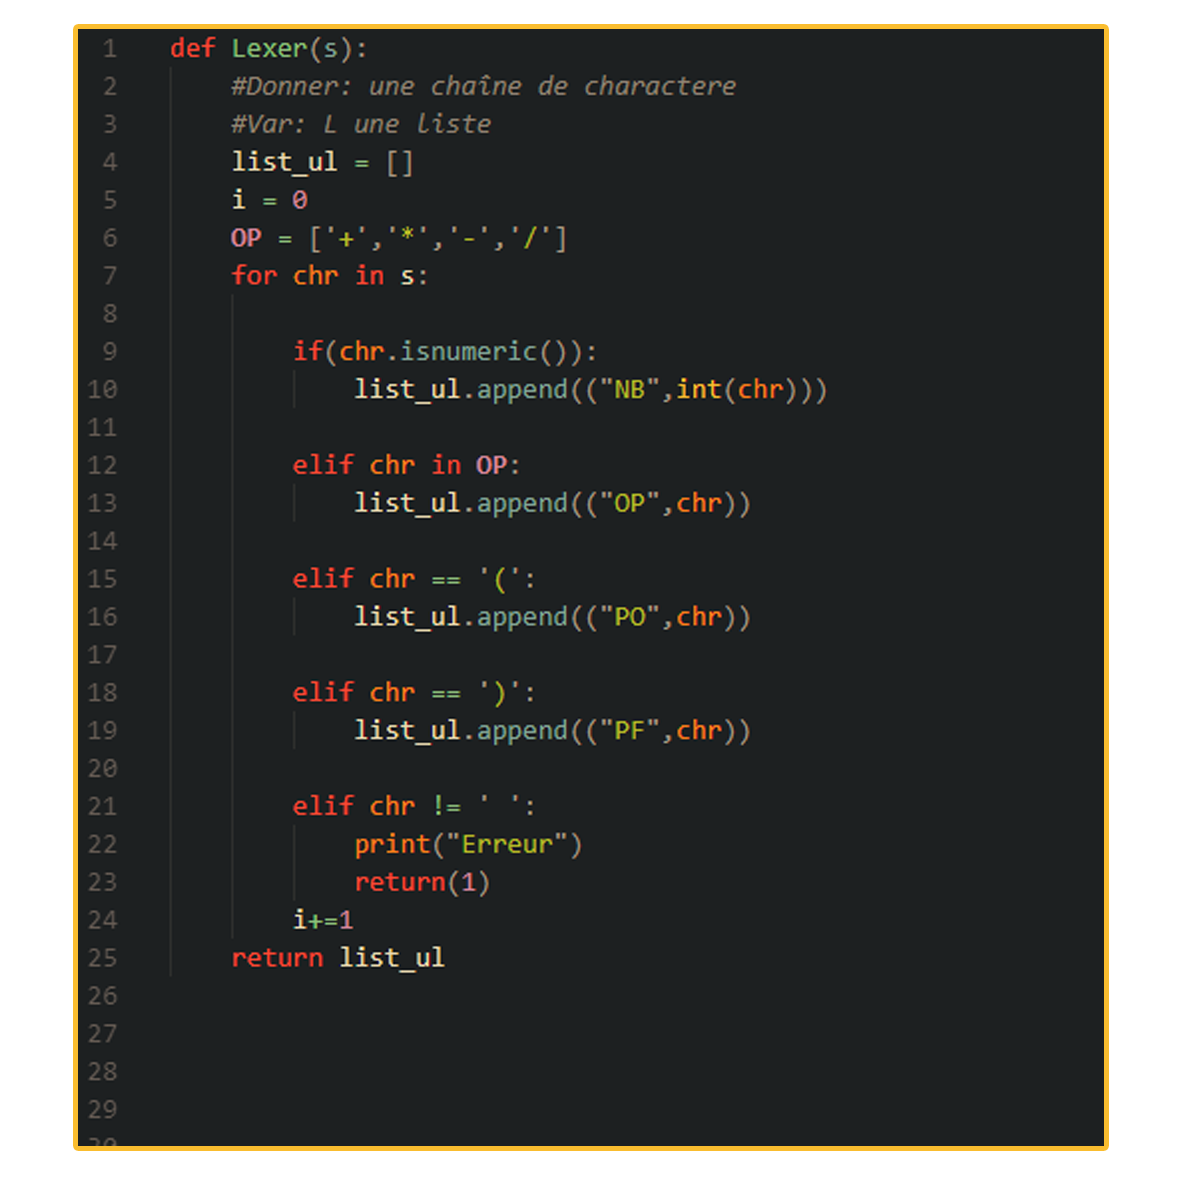
\includegraphics[width=10cm]{Lexer.png}\hspace*{\fill}
      \end{center}
      \subsection{Analyse syntaxique}
      Le but et de tranformer notre list d'uniter lexicale en arbre abstrait/syntaxique. Cette arbre devras refletais la stuture gramatical du langage, sachant qu'une grammaire se definit par un ensemble de regle appele production.
      On distingue deux type de syntaxe:\\
      \begin{enumerate}
        \item Terminaux, corespondant au lexeme du langage
        \item Non-Terminaux, qui sont des variable
      \end{enumerate}
      Une fois la grammaire $G$ definit, on sait que $G$ derive une expression $e$ si il exitse une suite fini de produit partant des symbole de depart et produisant $e$.\\
   \noindent\begin{minipage}{0.4\textwidth}% adapt widths of minipages to your needs
    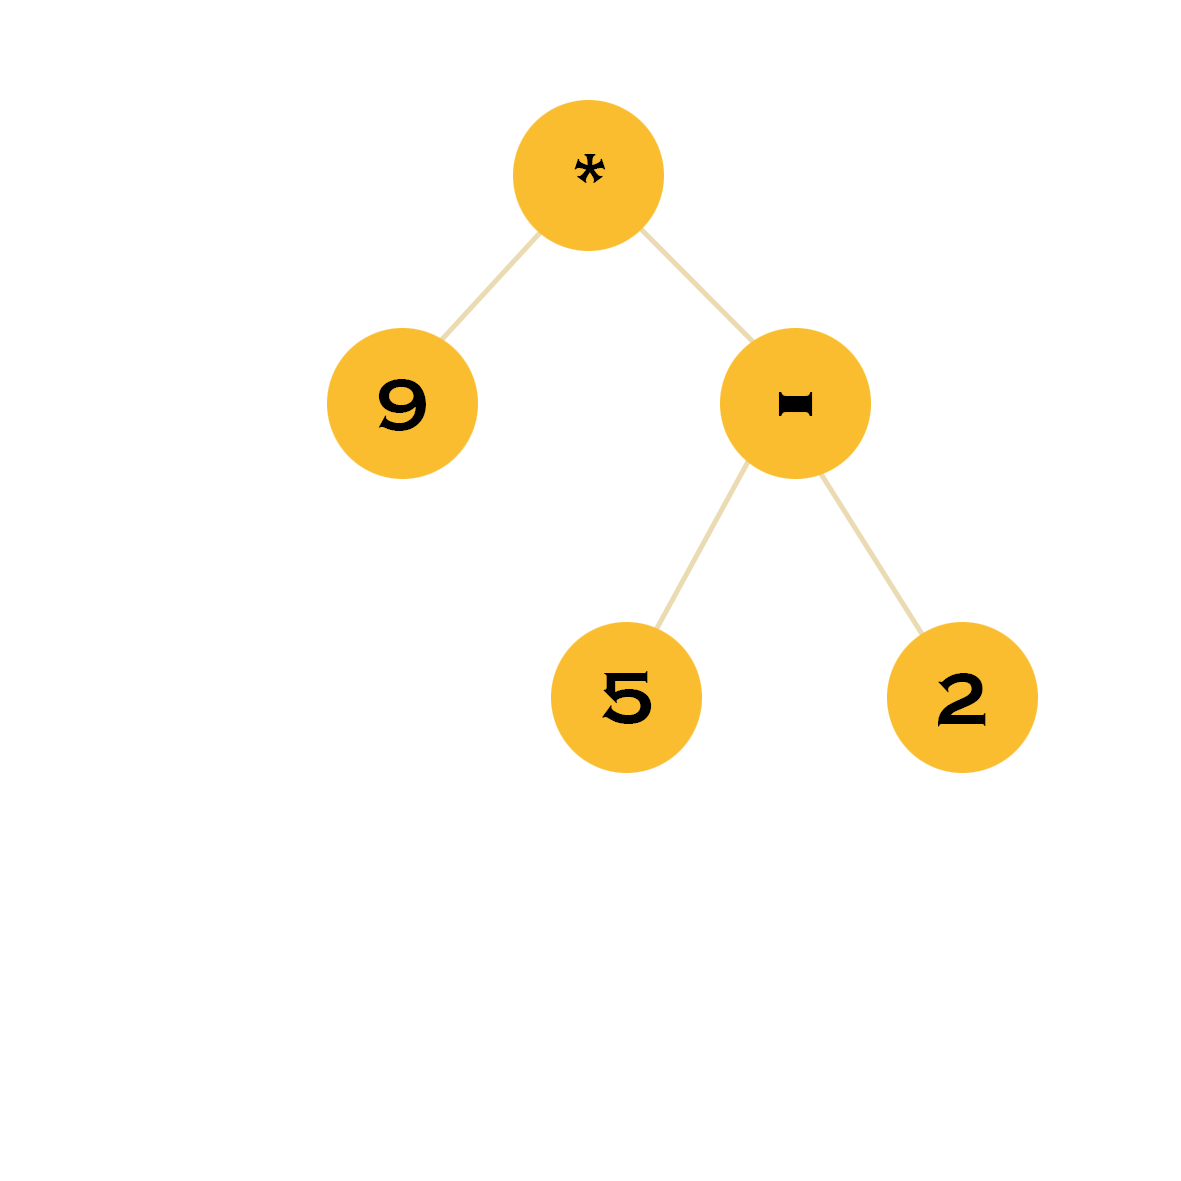
\includegraphics[width=\linewidth]{grap.png}
    \end{minipage}%
  \hfill%
  \begin{minipage}{0.5\textwidth}\raggedleft
    Prenon l'exemple de:\\
      9*(5-2)\\
      Expr-\> Expr Op Expr\\
  \end{minipage}
  \section{\color{OrangeHaf}Chapitre 2: Automate}
  %TODO Image classe
  \subsection{Langage}
  Pour resoudre les nombreux probleme que pose l'analyse lexicale des lanagge de programation nous allons etudier une partie 
  important de la sciences de l'informatique la theorie des langages et des automate.\\
      \textbf{Alphabet:}
        un alaphabet est un ensemble de fini, dont les element sont appele symbole ou lettre.
        \\
      \textbf{Mot:}
        soit $\sigma$ un alaphabet, un mot est une suite de simbole. par exemple: $w:w_1,w_2\ldots,w_n$ un mot sur $\sigma$.\\

        






\end{document}
